% =====================================================================
% Section 3 -- System architecture and methodology (ASMOE V2)
% Implementation: src/dataset.py, src/models/asmoe.py, src/losses.py, src/trainer.py
% =====================================================================
\section{Methods: ASMOE V2}
\label{sec:methodology}

ASMOE~V2 targets the bottlenecks identified in Section~\ref{sec:baseline_audit}
along three axes: \emph{data} (cleaning, leakage-free folds, leaf-centred inputs
at higher resolution), \emph{architecture} (heterogeneous experts aligned in a
shared space and fused by input-adaptive soft routing), and \emph{optimisation}
(two-stage refinement with discriminative learning rates and a supervised
contrastive objective). Figure~\ref{fig:asmoe_arch} gives an overview.

% Architecture diagram (hand-drawn): paper/figures_manual/asmoe_architecture.png,
% copied into paper/build/figures/ on every rebuild.
\begin{figure}[h]
\centering
\IfFileExists{figures/asmoe_architecture.pdf}{\includegraphics[width=\textwidth]{figures/asmoe_architecture.pdf}}{%
\IfFileExists{figures/asmoe_architecture.png}{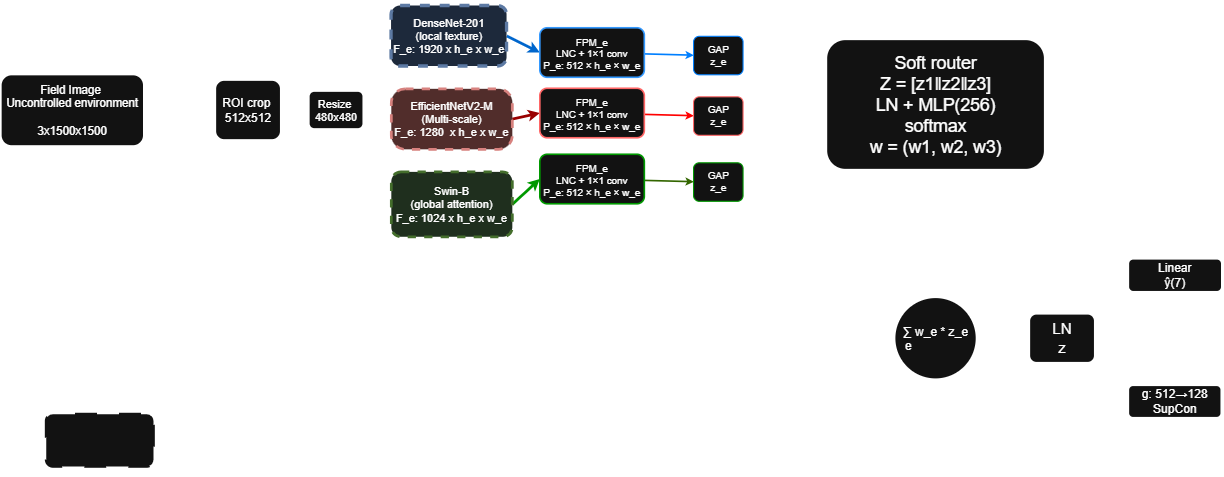
\includegraphics[width=\textwidth]{figures/asmoe_architecture.png}}{%
\fbox{\parbox{0.95\textwidth}{\centering\small
Input $x$ (ROI crop, $512^2$) $\;\rightarrow\;$
\{ DenseNet-201 @$512$ \,|\, EfficientNetV2-M @$480$ \,|\, Swin-B @$384$ \}
$\;\rightarrow\; F_e$ $\;\rightarrow\;$ FPM$_e$: LN $+$ $1{\times}1$ Conv $\rightarrow P_e\in\mathbb{R}^{512\times h_e\times w_e}$
$\;\rightarrow\;$ GAP $\rightarrow z_e$ \\[3pt]
$[z_1\Vert z_2\Vert z_3] \rightarrow$ MLP $\rightarrow$ softmax $\rightarrow w$
$\;\rightarrow\; z=\sum_e w_e z_e \;\rightarrow\;$ Linear $\rightarrow \hat{y}$
\quad and \quad $z\rightarrow g(\cdot)\rightarrow$ SupCon}}}}
\caption{ASMOE~V2 overview. Each expert sees the image at its native resolution;
the Feature Projection Module (FPM) aligns heterogeneous feature maps; the soft
router produces per-image expert weights.}
\label{fig:asmoe_arch}
\end{figure}

\subsection{Data curation and leakage-free cross-validation}
\label{sec:method_data}

Let $\mathcal{D}=\{(x_i,y_i)\}_{i=1}^{N}$ be the raw collection. We compute the
SHA-256 digest $s_i$ and a 64-bit difference hash $d_i$ of each file, and apply
three rules:
(i) every exact-duplicate group $\{i: s_i = s\}$ whose labels disagree is removed
entirely, since its ground truth is undefined;
(ii) within label-consistent exact-duplicate groups only one copy is kept;
(iii) surviving images with $\mathrm{Ham}(d_i,d_j)\le\tau$ ($\tau=2$) are joined
by union-find into one \emph{group} $g_i$. Cross-label near-duplicates, if any,
are removed like rule~(i). Folds are produced by
\texttt{StratifiedGroupKFold}($K{=}5$), which keeps class proportions while
guaranteeing $g_i=g_j \Rightarrow \mathrm{fold}(i)=\mathrm{fold}(j)$. The code
checks this invariant explicitly. All models in this paper, including the
re-trained baselines, share one fixed split.

\paragraph{Leaf ROI cropping.}
Field photographs contain soil, hands, sky and neighbouring plants. We build a
foliage-and-lesion mask
\begin{equation}
M = \underbrace{[\,2G-R-B > 0.05\,]}_{\text{excess green}}
\;\lor\; [\,H\in[35^\circ,170^\circ],\,S>0.18\,]
\;\lor\; \underbrace{[\,H\in[5^\circ,35^\circ),\,S>0.25\,]}_{\text{chlorosis / necrosis}},
\end{equation}
gated by $V>0.12$, smoothed with a $5{\times}5$ median filter. We take the 2nd--98th
percentile extent of $M$, add an 8\,\% margin and square it. Including
yellow-brown hues prevents necrotic lesions, the most informative pixels, from
being cropped away. If the mask covers less than 5\,\% of the image, or the box
would cover less than 15\,\% of it, the full frame is kept. Crops are cached once
at 640\,px on the longer side.

\paragraph{Resolution.}
Inputs are loaded at $512\times512$ (vs.\ $224$ in all legacy runs), and each
expert resamples them to its pre-training resolution (512, 480, 384). At
$512$\,px a 2\,mm lesion on a 10\,cm leaflet spans $\approx$10 pixels instead of
$\approx$4.

\paragraph{Lesion-preserving augmentation.}
Training uses horizontal and vertical flips, rotation $\mathcal{U}(-20^\circ,20^\circ)$,
affine translation ($\pm5\,\%$), scale ($[0.9,1.1]$) and shear ($\pm5^\circ$), and
ColorJitter (brightness and contrast $0.15$). CutMix~\cite{yun2019cutmix} is removed
(Section~\ref{sec:audit_cutmix}). On half of the mini-batches we apply mild MixUp~\cite{zhang2018mixup}
with $\lambda\sim\mathrm{Beta}(0.2,0.2)$ and $\lambda\leftarrow\max(\lambda,1-\lambda)$,
so the dominant image always contributes at least half of the pixels and the
label:
\begin{equation}
\tilde{x} = \lambda x_a + (1-\lambda)x_b,\qquad
\tilde{q} = \lambda\, q_a + (1-\lambda)\, q_b,
\end{equation}
where $q$ are label-smoothed one-hot targets ($\epsilon=0.05$).

\subsection{Heterogeneous experts}
\label{sec:method_experts}

Each expert $E_e$ is chosen for a different inductive bias that matches one of
the observed confusions:

\begin{itemize}
  \item \textbf{Local texture, DenseNet-201}~\cite{huang2017densenet} (or ConvNeXt-B in the large
  variant). Dense connectivity reuses low-level features in every block, so
  fine texture such as sporulation, frass and lesion rims, which separates Pest
  from Fungi, reaches the classifier without being washed out by depth.
  \item \textbf{Multi-scale, EfficientNetV2-M/L}~\cite{tan2021effnetv2}. Compound scaling and
  Fused-MBConv stages provide receptive fields from a few pixels to the whole
  leaf. This matters because lesion size varies by an order of magnitude between
  early and late infections.
  \item \textbf{Global attention, Swin-B/L}~\cite{liu2021swin}. Shifted-window self-attention
  relates distant regions, such as a mosaic pattern spread over the leaf or
  leaf-roll curvature. This is the evidence needed for Virus vs.\ Healthy, where
  no single local patch is diagnostic.
\end{itemize}

All experts are initialised from ImageNet-21k/1k weights (timm). For an input
$x$, expert $e$ resamples it to its own resolution $r_e$ and returns a feature map
$F_e = E_e(\mathrm{resize}(x, r_e)) \in \mathbb{R}^{C_e\times h_e\times w_e}$, with
$C_e\in\{1920, 1280, 1024\}$. Token outputs of the transformer are reshaped to a
spatial map.

\subsection{Feature Projection Module}
\label{sec:method_fpm}

The experts differ in channel count, spatial size and activation statistics
(BatchNorm-ReLU vs.\ LayerNorm-GELU). Before any fusion, the FPM maps each of them
into a shared $D$-dimensional space ($D=512$):
\begin{equation}
P_e = W_e * \mathrm{LN}_C(F_e) + b_e,\qquad
\mathrm{LN}_C(F)_{:,u,v} = \gamma \odot \frac{F_{:,u,v}-\mu_{u,v}}{\sigma_{u,v}} + \beta,
\end{equation}
where $\mathrm{LN}_C$ normalises across channels at every spatial location and
$W_e\in\mathbb{R}^{D\times C_e\times1\times1}$ is a pointwise convolution. Per-location
normalisation removes the scale mismatch between CNN and transformer features
while keeping the spatial layout, which Grad-CAM later uses. The expert descriptor
is
\begin{equation}
z_e = \frac{1}{h_e w_e}\sum_{u,v} P_e[:,u,v] \in \mathbb{R}^{D}.
\end{equation}

\subsection{Input-adaptive soft routing}
\label{sec:method_router}

Let $Z=[z_1\Vert\dots\Vert z_E]\in\mathbb{R}^{ED}$. The gating network is a two-layer
MLP followed by a temperature-scaled softmax:
\begin{equation}
w = \mathrm{softmax}\!\left(\frac{W_2\,\delta\!\big(W_1\,\mathrm{LN}(Z)+b_1\big)+b_2}{T}\right)\in\Delta^{E-1},
\end{equation}
with $\delta$ the GELU, $W_1\in\mathbb{R}^{256\times ED}$, dropout $0.1$ and $T=1$.
$W_2$ and $b_2$ are zero-initialised, so training starts from uniform routing
$w_e=1/E$ and moves away from it only when the data support it. The fused
representation and prediction are
\begin{equation}
z = \mathrm{LN}\Big(\sum_{e=1}^{E} w_e\, z_e\Big),\qquad
\hat{y} = \mathrm{softmax}(W_c\, z + b_c),
\end{equation}
with a single linear classifier $W_c\in\mathbb{R}^{7\times D}$. Unlike sparse
top-$k$ MoE, all experts contribute to every sample. This is affordable with
$E=3$, and the routing stays differentiable without auxiliary noise. To prevent
routing collapse onto one expert we add an importance-balancing regulariser
\begin{equation}
\mathcal{L}_{\mathrm{bal}} = E\sum_{e=1}^{E}\bar{w}_e^{\,2} - 1,\qquad
\bar{w}_e = \frac{1}{B}\sum_{i=1}^{B} w_{ie},
\end{equation}
which is zero for uniform batch-level usage and still allows strong per-image
specialisation.

\subsection{Training objective}
\label{sec:method_loss}

\paragraph{Weighted classification loss.}
With class counts $n_c$ in the training fold, $\alpha_c \propto n_c^{-1/2}$
(normalised to mean 1). The classification term is a soft-target weighted
cross-entropy,
\begin{equation}
\mathcal{L}_{\mathrm{cls}} = -\sum_c \alpha_c\, q_c \log p_c .
\end{equation}
Square-root weights are a milder form of inverse-frequency weighting. They were
the best option in the legacy policy screen and cause fewer minority false
positives (Section~\ref{sec:audit_imbalance}).

\paragraph{Supervised contrastive loss.}
Re-weighting moves the decision boundaries but does not separate the classes in
feature space. For the Pest/Fungi/Phytophthora cluster we therefore add the
supervised contrastive loss of Khosla \emph{et al.}~\cite{khosla2020supcon} on a projection
$h_i = g(z_i)/\lVert g(z_i)\rVert$, $g:\mathbb{R}^{512}\!\to\!\mathbb{R}^{128}$:
\begin{equation}
\mathcal{L}_{\mathrm{SC}} = \sum_{i\in I}\frac{-1}{|P(i)|}\sum_{p\in P(i)}
\log\frac{\exp(h_i^{\top}h_p/\tau)}{\sum_{a\in A(i)}\exp(h_i^{\top}h_a/\tau)},
\end{equation}
where $A(i)$ are all other samples in the batch, $P(i)=\{p\in A(i): y_p=y_i\}$ and
$\tau=0.07$. Anchors without positives are skipped, and the term is applied only
to non-MixUp batches, where labels are pure. It pulls images of the same class
together and pushes the confused pairs apart.

\paragraph{Total loss.}
\begin{equation}
\mathcal{L} = \mathcal{L}_{\mathrm{cls}} + \lambda_{\mathrm{SC}}\,\mathcal{L}_{\mathrm{SC}} + \lambda_{\mathrm{bal}}\,\mathcal{L}_{\mathrm{bal}},
\qquad \lambda_{\mathrm{SC}}=0.1,\; \lambda_{\mathrm{bal}}=0.01.
\end{equation}

\subsection{Two-stage refinement}
\label{sec:method_twostage}

Training three large pretrained experts on fewer than 2{,}500 images from random
heads quickly distorts their features. We therefore use two stages.

\textbf{Stage 1: alignment} (5 epochs). All backbone parameters are frozen,
including BatchNorm running statistics. Only the FPMs, router, classifier and
contrastive head are trained (AdamW, $\eta_{\mathrm{head}}=3\times10^{-4}$, cosine
decay). The randomly initialised layers learn to read the pretrained features
before any gradient reaches the backbones.

\textbf{Stage 2: refinement} (up to 40 epochs). All parameters are unfrozen with
discriminative learning rates, $\eta_{\mathrm{backbone}}=1\times10^{-5}$ and
$\eta_{\mathrm{head}}=3\times10^{-4}$, a 2-epoch linear warm-up and cosine
annealing to 1\,\% of the peak. Weight decay is 0.05 and gradients are clipped at
norm 1. We use automatic mixed precision (bf16 where supported, otherwise fp16
with loss scaling), gradient checkpointing, a micro-batch of 8 with 4-step
accumulation (effective batch 32) and an exponential moving average of the
weights (decay $0.999$).

\textbf{Model selection.} After every epoch we evaluate on the held-out fold
with horizontal-flip test-time augmentation. We keep the checkpoint with the
highest Macro-F1 and stop after 8 epochs without improvement in Stage~2. Because
the selection uses the validation fold, the 5-fold CV estimate is
selection-informed, as it was in the legacy campaign. We state this caveat with
every result.

\subsection{Evaluation protocol}
\label{sec:method_eval}

For every fold $k$ we compute accuracy, Macro-F1, weighted F1, Matthews
correlation coefficient (MCC), per-class precision, recall and F1, and the
confusion matrix. Tables report mean $\pm$ sample standard deviation over the five
folds, and confusion matrices are pooled. The legacy models are evaluated on the
same group-aware folds. Explanations are produced with routing-weighted
Grad-CAM~\cite{selvaraju2017gradcam},
\begin{equation}
\mathrm{CAM}_e = \mathrm{ReLU}\Big(\sum_k \alpha^e_k P_e^{k}\Big),\quad
\alpha^e_k = \frac{1}{h_e w_e}\sum_{u,v}\frac{\partial \hat{y}_c}{\partial P_e^{k}[u,v]},\quad
\mathrm{CAM} = \sum_e w_e\,\mathrm{up}(\mathrm{CAM}_e),
\end{equation}
and summarised by the \emph{lesion-focus ratio}, the share of CAM mass falling
inside the foliage-and-lesion mask $M$.
